% We switch to portrait mode. This works as advertised.
\documentclass[xcolor=table]{beamer}
\usepackage[orientation=portrait, size=a0, scale=1]{beamerposter}

\usepackage[utf8]{inputenc}
\usepackage[british]{babel}
\usepackage[super]{nth}

%math
\usepackage{amsmath,mathtools}
\usepackage{amssymb}

%chemistry
\usepackage[version=3]{mhchem}
\usepackage{chemfig}
\usepackage{setspace}

%physics
\usepackage[separate-uncertainty = true]{siunitx}

%\usetheme{Boadilla}
%\usecolortheme{rose}
%\usecolortheme{crane}
%\usefonttheme{structuresmallcapsserif}
%\setbeamertemplate{navigation symbols}{}

\mode<presentation>{\usetheme{ilm}}

%\definecolor{Main}{rgb}{0.74, 0.13, 0.19}
\colorlet{Main}{ilmorange}
%\definecolor{Accent1}{rgb}{0.76,0.36,0.13}
\colorlet{Accent1}{ilmcolor}
%\definecolor{Accent2}{rgb}{0.54,0.1,0.4}
\colorlet{Accent2}{ilmcolor!65!black}



% see documentation for a0poster class for the size options here
\let\Textsize\normalsize
\def\Norulehead#1{\noindent\hbox to \hsize{\hfil\LARGE\textcolor{Main}{\textbf{#1}}}\bigskip}
\def\Head#1{\Norulehead{\hrulefill #1}}
\def\LHead#1{\noindent{\Large \color{Accent2}\textbf{#1}}\smallskip}
\def\affiliation#1{\Large \textcolor{Accent2}{\textit{#1}}\smallskip}
\def\Subhead#1{\noindent{\large\color{Accent1}\textbf{#1}}}
\def\Title#1{\noindent{\veryHuge\color{Main}\raggedright\textsf{\textbf{#1}}}}

\setbeamertemplate{headline}{%
	%logo sponsors
	\let\mydim\relax
	\newlength\mydim
	\setlength{\mydim}{0.75cm}
	\rule[-.3\baselineskip]{0pt}{4.5cm}
	\hfill\pgfuseimage{cnrs-logo}\hspace*{\mydim}\pgfuseimage{ucbl-logo}\hspace*{\mydim}
	
\includegraphics[height=3cm]{presentation/ENS_Lyon.pdf}\hspace*{\mydim}
	\pgfuseimage{univlyon-logo}\hspace*{\mydim}
	
\includegraphics[height=4cm]{presentation/invest-avenir.pdf}\hspace*{\mydim}
	\includegraphics[height=4cm,clip=true, trim=6mm 14mm 6mm 0]{../Yaourt/NEW-Logo-ERC-OUTLINE}\hspace*{\mydim}
	
\includegraphics[height=3cm]{presentation/frama.png}\hspace*{\mydim}
	
\includegraphics[height=4cm]{presentation/ICL}\hspace*{\mydim}
}

% The textpos package is necessary to position textblocks at arbitary 
% places on the page.
\usepackage[absolute,overlay,showboxes
]{textpos}
% Set up the grid
%
% Note that [40mm,40mm] is the margin round the edge of the page --
% it is _not_ the grid size. That is always defined as 
% PAGE_WIDTH/HGRID and PAGE_HEIGHT/VGRID. In this case we use
% 15 x 25. This gives us a wide central column for text (7 grid
% spacings) and two narrow columns (3 each) at each side for 
% pictures, separated by 1 grid spacing.
%
% Note however that texblocks can be positioned fractionally as well,
% so really any convenient grid size can be used.
%
\TPGrid[40mm,40mm]{15}{25}  % 3 - 1 - 7 - 1 - 3 Columns

% Mess with these as you like
\parindent=0pt
%\parindent=1cm
\parskip=0.5\baselineskip

\usepackage{paralist}

% Allow the usage of graphics (.jpg, .png, etc.) in the document
\usepackage{graphicx}
\usepackage{tikz}
\usetikzlibrary{arrows,shapes,backgrounds, calc, positioning, topaths,chains, intersections, decorations.markings, decorations.text, shapes.geometric, matrix,patterns,mindmap,fit}
%\usetikzlibrary{positioning, patterns,topaths,chains,matrix}

\usepackage{pgfplots}
\usepackage{pgfplotstable}
\pgfplotsset{compat=1.9}
\usepgfplotslibrary{fillbetween}
\usepgfplotslibrary{groupplots}
\usepgfplotslibrary{external}
\makeatletter
\newcommand*{\overlaynumber}{\number\beamer@slideinframe}
\tikzset{
  beamer externalizing/.style={%
    execute at end picture={%
      \tikzifexternalizing{%
        \ifbeamer@anotherslide
        \pgfexternalstorecommand{\string\global\string\beamer@anotherslidetrue}%
        \fi
      }{}%
    }%
  },
  external/optimize=false
}
\let\orig@tikzsetnextfilename=\tikzsetnextfilename
\renewcommand\tikzsetnextfilename[1]{\orig@tikzsetnextfilename{#1-\overlaynumber}}
\makeatother

%\tikzset{every picture/.style={beamer externalizing}}
%\tikzexternalize
%\tikzsetexternalprefix{fig_poster/}



\begin{document}
\begin{frame}
%title
\begin{textblock}{15}(0,0.8)

{\setlength{\baselineskip}{2.75\baselineskip}\hspace*{0.3\paperwidth}\Title{
Ion pairing controls rheological properties of ``processionary'' polyelectrolyte hydrogels
}\hfill \textit{Soft Matter} 2016, \textbf{12}, 9749-9758\par}

\centering

\vspace{0.5cm}
\LHead{Hassan Srour,\textit{$^{1}$} Martien Duvall Deffo Ayagou,\textit{$^{1}$} Thi Thanh-Tam Nguyen,\textit{$^{1}$}, Nicolas Taberlet,\textit{$^{2}$} S\'{e}bastien Manneville,\textit{$^{2}$}\\ Chantal Andraud,\textit{$^{1}$} Cyrille Monnereau,$^{\ast}$\textit{$^{1}$} and Mathieu Leocmach$^{\ast}$\textit{$^{3}$
}}\hspace{0.1\paperwidth}\texttt{\color{Main}\Large mathieu.leocmach@univ-lyon1.fr}\\

\affiliation{$^{1}$ Univ Lyon, Ens de Lyon, Universit\'e Claude Bernard Lyon 1, CNRS,
Laboratoire de Chimie, F-69342 Lyon, France.\\
$^{2}$ Univ Lyon, Ens de Lyon, Universit\'e Claude Bernard Lyon 1, CNRS,
Laboratoire de Physique, F-69342 Lyon, France.\\
$^{3}$ Univ Lyon, Universit\'e Claude Bernard Lyon 1, CNRS, Institut Lumi\`ere Mati\`ere, F-69622, VILLEURBANNE}
\end{textblock}%title


\begin{textblock}{4}(0,4)
	\Head{Cation terminated polyanion}
	\tikzsetnextfilename{polymerisation}%
	\let\mrad\relax%
	\newlength\mrad%
	\setlength{\mrad}{1ex}%
	% The face style, can be changed
	\tikzset{face/.style={
		shape=circle,minimum size=2\mrad,shading=radial,outer sep=0pt,
	    inner color=white!50!yellow,outer color= yellow!70!orange
		}}%
	\begin{tikzpicture}
		\foreach \i [evaluate=\i as \dist using \i*0.45] in {0,1,2}{
			\begin{scope}[xshift=\dist\textwidth]
			%face
			\begin{scope}[face/.style={
		shape=circle,minimum size=2\mrad,shading=radial,outer sep=0pt,
	    inner color=white!50!yellow,outer color= yellow!70!orange
		}]
\node[face,inner color=white!50!ilmcolor,outer color= ilmcolor!90!black] (emoticon) {};
			%% The eyes are fixed.
			\draw[fill=white] 
				(-0.5\mrad,0ex) ..controls (-0.25\mrad,0.1\mrad)and(0.25\mrad,0.1\mrad)..
		        (0.5\mrad,0.0pt) ..controls (0.75\mrad,0.75\mrad)and(0.1\mrad,0.85\mrad)..
		        (0pt,0.2\mrad) ..controls (-0.1\mrad,0.85\mrad)and(-0.75\mrad,0.75\mrad)..
		        (-0.5\mrad,0pt)--cycle;
			%% standard pupils
			\node[fill, ellipse,inner xsep=0.075\mrad, inner ysep=0.0375\mrad, rotate=80] at (0.25\mrad,0.25\mrad) {};
			\node[fill, ellipse,inner xsep=0.075\mrad, inner ysep=0.0375\mrad, rotate=100] at (-0.25\mrad,0.25\mrad) {};
			%% mouth
			\draw[thick,line cap=round] (-0.5\mrad,-0.5\mrad)
			     ..controls (-0.25\mrad,-0.75\mrad)and(0.25\mrad,-0.75\mrad)..(0.5\mrad,-0.5\mrad);
\end{scope}
;
			%% horns
			\draw[every node/.style={shape=circle,inner sep=0.2\mrad,shading=radial,inner color=white!50!ilmcolor,outer color= ilmcolor!90!black}] (emoticon.70) -- ++(70:0.4\mrad) node{} (emoticon.110) -- ++(110:0.4\mrad) node{};
			%\draw ( emoticon.80)..controls ( 0.3\mrad,1.2\mrad)..(0.5\mrad,1.25\mrad)
			      %..controls ( 0.4\mrad,1.15\mrad)..(emoticon.70);
			%\draw (emoticon.100)..controls (-0.3\mrad,1.2\mrad)..(-0.5\mrad,1.25\mrad)
			      %..controls (-0.4\mrad,1.15\mrad)..(emoticon.110);
			%body segments
			\ifthenelse{\i=0}{}{
			\foreach \x in {0,2,...,10}{
				\node[face,inner color=white!50!gray,outer color= gray!90!black, left=\x\mrad of emoticon] (monomer){};
				%legs
				\ifthenelse{\i=1}{}{
					\draw[line width=0.25\mrad, ilmorange] (monomer.south) ++(0,0.5\mrad) to[bend left] +(0,-1\mrad);}
			};}
			\ifthenelse{\i=1}{
				\draw[|-|] ($(monomer.west)+(0,-1.5\mrad)$) -- ($(emoticon.west)+(0,-1.5\mrad)$) node[midway,below, font=\scriptsize] {$N_0$};
			}{}
			\end{scope}
			};
			%arrows
			\draw[-stealth, thick] ++(3\mrad,0) -- +(6\mrad,0) node[midway, above=0.2\mrad, face,inner color=white!50!gray,outer color= gray!90!black]{} node[midway, below, font=\scriptsize]{ATRP};
			\draw[-stealth, thick] ++(0.45\textwidth,0) ++(3\mrad,0) -- +(6\mrad,0) coordinate[midway, above=0.2\mrad] (leg) node[midway, below, font=\scriptsize,text width=10\mrad,align=center]{post-functionalization};
			\draw[line width=0.25\mrad, ilmorange] (leg) to[bend right] +(0,1\mrad);
		\end{tikzpicture}

	\bigskip
	\tikzsetnextfilename{polymerisation_PImBr}%
	\definesubmol{head}{(-[::-105,,,,ilmcolor])(-[::-15,,,,ilmcolor])-[::60,,,,ilmcolor](=[::60,,,,ilmcolor]\textcolor{ilmcolor}{O})-[::-60,,,,ilmcolor]\textcolor{ilmcolor}{O}-[::-60,,,,ilmcolor]-[::60,,,,ilmcolor]-[::60,,,,ilmcolor]}
\definesubmol{mono}{-[::-60,,,,gray](=[,,,,gray]\textcolor{gray}{O})-[::-60,,,,gray]\textcolor{gray}{O}-[::60,,,,gray]-[,,,,gray]-[::-60,,,,gray]}
\tikzsetnextfilename{polymerisation_PImBr}
\begin{tikzpicture}[every node/.style={font=\tiny\setatomsep{1.5em}}]
	\node (init) {\chemfig{Br-[:-30]!{head}\textcolor{ilmcolor}{P}|\textcolor{ilmcolor}{O_3}Et_2}};
	
	\node[below left=5\baselineskip and 0 of init.east] (POH) {%
	\chemfig{[:-30]-[@{left,0.25}](%
		!{mono}OH%
		)-[::60,,,,gray]-[@{right,0.25}]!{head}\textcolor{ilmcolor}{P}|\textcolor{ilmcolor}{O_3}Et_2}%
	};
	\node[below right=-0.6em and -0.25em of POH.base west] {$\prescript{}{N_0}{\left[\vrule height 1em depth 0.25em width 0pt\hspace{1.75em}\right]}$};
	\node[below right=-0.6em and -0.25em of POH.base west] {};
	
	\node[right=0.1\textwidth of init.base east, anchor=base west] (PBr) {%
	\chemfig{[:-30]-[@{left,0.25}](%
		!{mono}Br%
		)-[::60,,,,gray]-[@{right,0.25}]!{head}\textcolor{ilmcolor}{P}|\textcolor{ilmcolor}{O_3^{2-}}}%
	};
	\node[below right=-0.6em and -0.25em of PBr.base west] {$\prescript{}{N_0}{\left[\vrule height 1em depth 0.25em width 0pt\hspace{1.75em}\right]}$};
	
	\node[right=\textwidth of init.base-|POH.west, anchor=base east] (PNuBr) {%
	\chemfig{[:-30]-[@{left,0.25}](%
		!{mono}\textcolor{ilmorange}{N}|^{\color{ilmorange}+}*5(=[,,,,thick, ilmorange]-[,,,,thick, ilmorange]\textcolor{ilmorange}{N}(-[,,,,thick, ilmorange])-[,,,,thick, ilmorange]=[,,,,thick, ilmorange]-[,,,,thick, ilmorange])(-[0,2,,,draw=none]Br^{-})
		)-[::60,,,,gray]-[@{right,0.25}]!{head}\textcolor{ilmcolor}{P}|\textcolor{ilmcolor}{O_3^{2-}}}%
	};
	\node[below right=-0.6em and -0.25em of PNuBr.base west] {$\prescript{}{N_0}{\left[\vrule height 1em depth 0.25em width 0pt\hspace{1.75em}\right]}$};
	
	\draw[-stealth, thick] (init.south-|POH.north) -- (POH) node[midway, left=0, -]{\chemfig{[:-30]=[,,,,gray]!{mono}OH}} node[midway, right=0, text width=0.13\textwidth, align=center]{\ce{CuBr}\linebreak 4-4'-bipyridine\linebreak \SI{85}{\celsius}};
	\draw[-stealth, thick] (POH) -| (PBr) node[pos=0.25, above]{\ce{TMS-Br}} node[pos=0.25, below, sloped, text width=0.2\textwidth, align=center]{\ce{CH2Cl2}\linebreak \SI{85}{\celsius}};
	\draw[-stealth, thick] (PBr) -- (PBr-|PNuBr.west) node[midway, above,align=center,-]{\chemfig[thick, ilmorange]{[2]*5(-N(-)-=N-=)}} node[midway, below, text width=0.2\textwidth, align=center]{THF\linebreak \SI{85}{\celsius}};;
	\node[anchor=south east] at (POH.south east) {\ce{POH}};
	\node[anchor=south east] at (PBr.south east) {\ce{PBr}};
	\node[anchor=south east] at (PNuBr.south east) {\ce{PIm+Br-}};
	\node[anchor=south east, font=\footnotesize] at (POH.south-|PNuBr.east) {$N_0=70$ from NMR};
\end{tikzpicture}
\end{textblock} %synthesis

\begin{textblock}{2.5}(5,4)
\Head{Yield stress fluid}
\Subhead{Reversible gel}

Herschel-Bulkley law \hfill$\sigma =\sigma_c + A \dot{\gamma}^n$
\tikzsetnextfilename{flowcurves}%
\begin{tikzpicture}
    \let\mrad\relax%
	\newlength\mrad%
	\setlength{\mrad}{0.5em}%
% The face style, can be changed
	\tikzset{face/.style={
		shape=circle,minimum size=2\mrad,shading=radial,outer sep=0pt,
	    inner color=white!50!yellow,outer color= yellow!70!orange
		}}%
\let\drawcaterpillar\relax
\newcommand\drawcaterpillar{
			%face
			\begin{scope}[face/.style={
		shape=circle,minimum size=2\mrad,shading=radial,outer sep=0pt,
	    inner color=white!50!yellow,outer color= yellow!70!orange
		}]
\node[face,inner color=white!50!ilmcolor,outer color= ilmcolor!90!black] (emoticon) {};
			%% The eyes are fixed.
			\draw[fill=white] 
				(-0.5\mrad,0ex) ..controls (-0.25\mrad,0.1\mrad)and(0.25\mrad,0.1\mrad)..
		        (0.5\mrad,0.0pt) ..controls (0.75\mrad,0.75\mrad)and(0.1\mrad,0.85\mrad)..
		        (0pt,0.2\mrad) ..controls (-0.1\mrad,0.85\mrad)and(-0.75\mrad,0.75\mrad)..
		        (-0.5\mrad,0pt)--cycle;
			%% standard pupils
			\node[fill, ellipse,inner xsep=0.075\mrad, inner ysep=0.0375\mrad, rotate=80] at (0.25\mrad,0.25\mrad) {};
			\node[fill, ellipse,inner xsep=0.075\mrad, inner ysep=0.0375\mrad, rotate=100] at (-0.25\mrad,0.25\mrad) {};
			%% mouth
			\draw[thick,line cap=round] (-0.5\mrad,-0.5\mrad)
			     ..controls (-0.25\mrad,-0.75\mrad)and(0.25\mrad,-0.75\mrad)..(0.5\mrad,-0.5\mrad);
\end{scope}

			
%body segments
			\foreach \x in {0,2,...,4}{
				\node[face,inner color=white!50!gray,outer color= gray!90!black, left=\x\mrad of emoticon] (monomer){};
				%legs
				\draw[line width=0.25\mrad, ilmorange] (monomer.south) ++(0,0.5\mrad) to[bend left] +(0,-1\mrad);
			};
}
\begin{loglogaxis}[
	name=ax,
	width=\textwidth-5em,
	height=6\baselineskip,
	xlabel=$\dot\gamma\,(\si{\per\second})$,
	ylabel={$\sigma$ (\si{\pascal)}},
	clip marker paths=true,
	scale only axis,
	]
	\addplot+[mark=o, ilmcolor] table[x=shear_rate, y=shear_stress] {data/PO3-P60-Im+-0pc-02-06-14_8pcw_flow curve_down.txt} node[pos=0, font=\scriptsize, inner xsep=0, below left=1em and 0]{8\% wt};
	\addplot+[mark=square, ilmcolor!60!black] table[x=shear_rate, y=shear_stress] {data/PO3-P60-Im+-0pc-02-06-14_22pcw_flow curve_down.txt} node[pos=1, font=\scriptsize, inner xsep=0, above right=0.2em and -0.5em]{22\% wt};
	\addplot+[ilmorange] table[x=shear_rate, y=shear_stress,skip coords between index={0}{20}] {data/Et-P60-Im+-0pc-21-05-14_10pcw_flow_curve_down.txt} node[pos=0, font=\scriptsize, inner xsep=0, right=0.8em]{10\% wt};
	\addplot[domain=2e-2:5e2]{0.47+1.19*x^0.7};
	\addplot[domain=2e-2:5e2]{7.5+15.1*x^0.62};
\end{loglogaxis}

\begin{scope}[shift=(ax.north), yshift=-2\mrad, xshift=-\mrad]
			\drawcaterpillar
			%% horns
			\draw[every node/.style={shape=circle,inner sep=0.2\mrad,shading=radial,inner color=white!50!ilmcolor,outer color= ilmcolor!90!black}] (emoticon.70) -- ++(70:0.4\mrad) node{} (emoticon.110) -- ++(110:0.4\mrad) node{};
\end{scope}
\begin{scope}[shift=(ax.south), yshift=2\mrad, xshift=-\mrad]
			\drawcaterpillar
\end{scope}
\end{tikzpicture}

\Subhead{Solution} if
\begin{itemize}
	\item ionic strength, pH
	\item non ionic head
\end{itemize}
$\Rightarrow$ Head-to-body ionic bonds

\textit{\footnotesize Srour et al. Macromol. Rapid Comm., 36, 55 (2015)}

\end{textblock} %Yield-stress fluid

\begin{textblock}{2.5}(8.5,4)
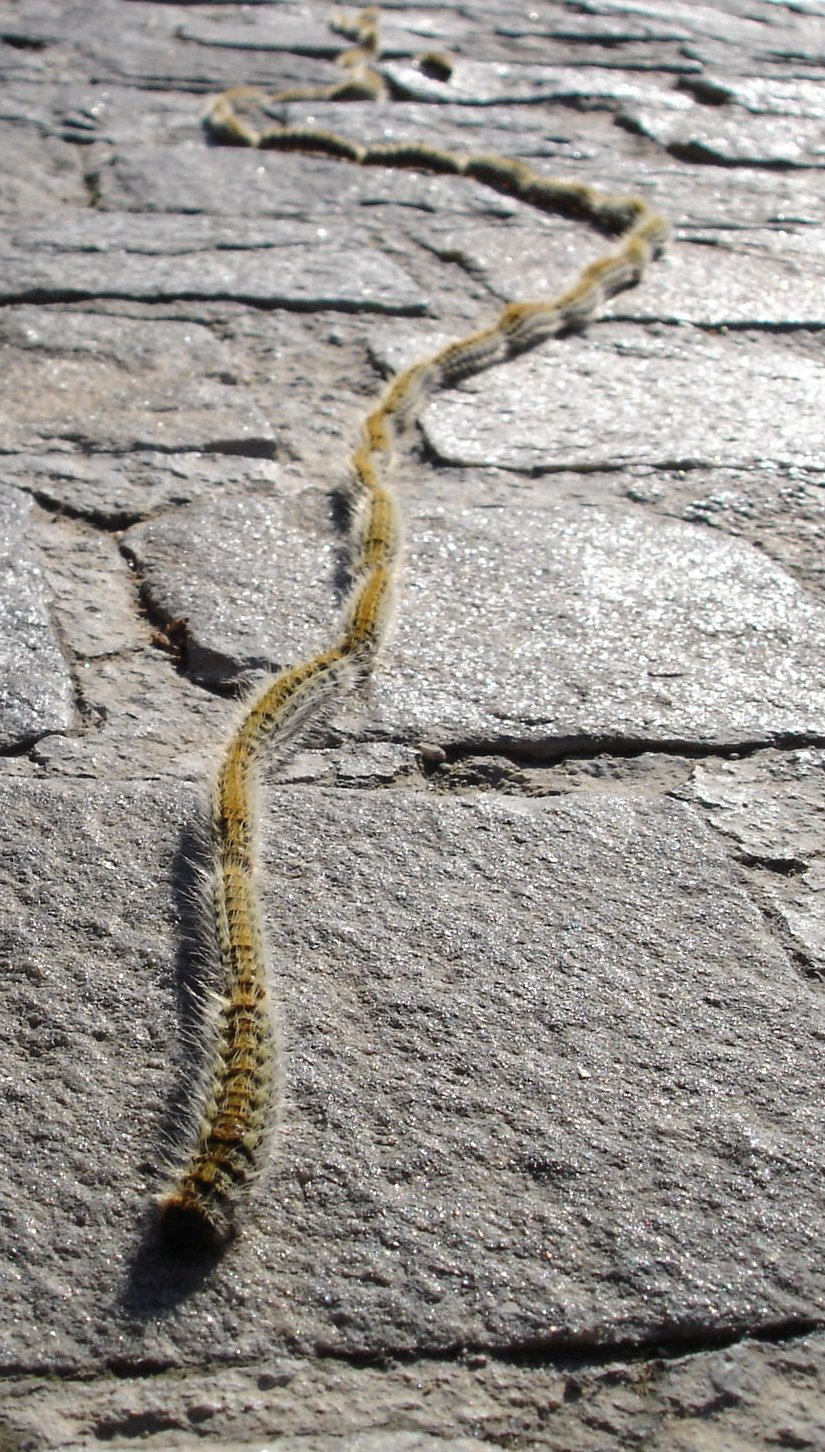
\includegraphics[width=\textwidth]{presentation/Thaumetopea_pityocampa_01.jpg}\\
	\vspace{-1.5em}\colorbox{lightgray}{\scriptsize Jürgen Appel on Wikimedia commons}
\end{textblock} %procession picture

\begin{textblock}{4}(0,8)
	\Head{Procession length}
	\[ G = \frac{c}{N}k_\mathrm{B}T \qquad \begin{array}{ll}
	\textcolor{Main}{c} & \text{monomer concentration}\\
	\textcolor{Main}{N} & \text{\# monomers between crosslinks}\\
	\end{array}\]
	$G\approx \SI{13}{\pascal}$\hfill$\Rightarrow$\hfill
	$N \approx 800 N_0$\hfill$\Rightarrow$\hfill
	800 chains between CL!
\end{textblock} %procession length

\begin{textblock}{5}(0,10)
	\Head{Postfunctionalisation}
	\tikzsetnextfilename{postfunc}%
	\let\mrad\relax%
	\newlength\mrad%
	\setlength{\mrad}{1ex}%
	% The face style, can be changed
	\tikzset{face/.style={
		shape=circle,minimum size=2\mrad,shading=radial,outer sep=0pt,
	    inner color=white!50!yellow,outer color= yellow!70!orange
		}}%
	\begin{tikzpicture}
		\foreach \i [evaluate=\i as \dist using (floor(\i/2))*0.4, evaluate=\i as \ys using 1.5*(\i-2*floor(\i/2))] in {1,2,3,4,5}{
			\begin{scope}[xshift=\dist\textwidth, yshift=\ys\baselineskip]
			
			%face
			\begin{scope}[face/.style={
		shape=circle,minimum size=2\mrad,shading=radial,outer sep=0pt,
	    inner color=white!50!yellow,outer color= yellow!70!orange
		}]
\node[face,inner color=white!50!ilmcolor,outer color= ilmcolor!90!black] (emoticon) {};
			%% The eyes are fixed.
			\draw[fill=white] 
				(-0.5\mrad,0ex) ..controls (-0.25\mrad,0.1\mrad)and(0.25\mrad,0.1\mrad)..
		        (0.5\mrad,0.0pt) ..controls (0.75\mrad,0.75\mrad)and(0.1\mrad,0.85\mrad)..
		        (0pt,0.2\mrad) ..controls (-0.1\mrad,0.85\mrad)and(-0.75\mrad,0.75\mrad)..
		        (-0.5\mrad,0pt)--cycle;
			%% standard pupils
			\node[fill, ellipse,inner xsep=0.075\mrad, inner ysep=0.0375\mrad, rotate=80] at (0.25\mrad,0.25\mrad) {};
			\node[fill, ellipse,inner xsep=0.075\mrad, inner ysep=0.0375\mrad, rotate=100] at (-0.25\mrad,0.25\mrad) {};
			%% mouth
			\draw[thick,line cap=round] (-0.5\mrad,-0.5\mrad)
			     ..controls (-0.25\mrad,-0.75\mrad)and(0.25\mrad,-0.75\mrad)..(0.5\mrad,-0.5\mrad);
\end{scope}

			%% horns
			\draw[every node/.style={shape=circle,inner sep=0.2\mrad,shading=radial,inner color=white!50!ilmcolor,outer color= ilmcolor!90!black}] (emoticon.70) -- ++(70:0.4\mrad) node{} (emoticon.110) -- ++(110:0.4\mrad) node{};
			%\draw ( emoticon.80)..controls ( 0.3\mrad,1.2\mrad)..(0.5\mrad,1.25\mrad)
			      %..controls ( 0.4\mrad,1.15\mrad)..(emoticon.70);
			%\draw (emoticon.100)..controls (-0.3\mrad,1.2\mrad)..(-0.5\mrad,1.25\mrad)
			      %..controls (-0.4\mrad,1.15\mrad)..(emoticon.110);
			%body segments
			
			\foreach \x in {0,2,...,8}{
				\node[face,inner color=white!50!gray,outer color= gray!90!black, left=\x\mrad of emoticon] (monomer){};
				%legs
				\ifthenelse{\i=3}{
					\draw[line width=0.25\mrad, ilmorange] (monomer.south) ++(0,0.5\mrad) to[bend left] +(0,-1\mrad);}{}
				\ifthenelse{\i=2}{
					\node[circle, inner sep=0.3\mrad, fill=ilmorange] at (monomer.south){};}{}
				\ifthenelse{\i=5}{
					\draw[line width=0.25\mrad, blue!80!black] (monomer.south) ++(0,0.5\mrad) to[bend left] +(0,-1\mrad);}{}
				\ifthenelse{\i=4}{
					\node[circle, inner sep=0.3\mrad, fill=blue!80!black] at (monomer.south){};}{}
			};
			\end{scope}
			};
			%arrows
			%\draw[-stealth, thick] ++(3\mrad,0) -- +(6\mrad,0) node[midway, above=0.2\mrad, face,inner color=white!50!gray,outer color= gray!90!black]{} node[midway, below, font=\scriptsize]{ATRP};
			\draw[-stealth, thick] ++(3\mrad,1.5\baselineskip) -- +(6\mrad,0) coordinate[midway, above=0.2\mrad] (leg) node[midway, below, font=\scriptsize,text width=10\mrad,align=center]{post-functionalization};
			\draw[line width=0.25\mrad, ilmorange] (leg) to[bend right] +(0,1\mrad);
			\draw[-stealth, thick] ++(3\mrad,0) -- +(6\mrad,0) node[midway, below=0.2\mrad, circle, inner sep=0.3\mrad, fill=ilmorange] (leg){};
			\draw[-stealth, thick] ++(0.425\textwidth,0) ++(3\mrad,0.75\baselineskip) -- +(6\mrad,0) coordinate[midway, above=0.2\mrad] (leg) node[midway, above, font=\scriptsize]{counterion} node[midway, below, font=\scriptsize,text width=10\mrad,align=center]{exchange};
		\end{tikzpicture}
	
	\tikzsetnextfilename{solubility}%
	\begin{tikzpicture}
\pgfdeclarelayer{background}
\pgfdeclarelayer{foreground}
\pgfsetlayers{background,main,foreground}
\node (PBr) {PBr} [->, level distance=9em, font=\footnotesize] 
	child [grow=-20] {node(PImBr) {\ce{P\textcolor{ilmorange}{\ce{Im+}}\textcolor{blue!80!black}{\ce{Br-}}}} [level distance=5em]
		child[grow=-30] {node(PImF) {\ce{P\textcolor{ilmorange}{\ce{Im+}}\textcolor{blue!80!black}{\ce{F-}}}}} 
		child[grow=east] {node(PImCl) {\ce{P\textcolor{ilmorange}{\ce{Im+}}\textcolor{blue!80!black}{\ce{Cl-}}}}} 
		child[grow=west] {node(PImI) {\ce{P\textcolor{ilmorange}{\ce{Im+}}\textcolor{blue!80!black}{\ce{I-}}}}}} 
	child [grow=-160] {node(PPyrBr) {\ce{P\textcolor{ilmorange}{\ce{Pyr+}}\textcolor{blue!80!black}{\ce{Br-}}}} [level distance=5em]
		child[grow=-30] {node(PPyrF) {\ce{P\textcolor{ilmorange}{\ce{Pyr+}}\textcolor{blue!80!black}{\ce{F-}}}}} 
		child[grow=east] {node(PPyrCl) {\ce{P\textcolor{ilmorange}{\ce{Pyr+}}\textcolor{blue!80!black}{\ce{Cl-}}}}} 
		child[grow=west] {node(PPyrI) {\ce{P\textcolor{ilmorange}{\ce{Pyr+}}\textcolor{blue!80!black}{\ce{I-}}}}}};
\begin{pgfonlayer}{background}
	\draw[lightgray, line width=0.3em, -stealth,rounded corners] (PImI.south) -- (PImBr.south) node[pos=0, below right] {Hoffmeister} -- (PImCl.south) -- (PImF);
	\draw[lightgray, line width=0.3em, -stealth,rounded corners] (PPyrI.south) -- (PPyrBr.south) node[pos=0, below right] {Hoffmeister} -- (PPyrCl.south) -- (PPyrF);
	\draw[ilmorange!25, line width=0.3em, -stealth,rounded corners] (PPyrI.base) -- (PPyrBr.base) -- (PPyrCl.base) -- (PImI.base) -- (PImBr.base);
\end{pgfonlayer}
	\foreach \x in {PImF,PImCl,PPyrF}{
	\draw[ilmcolor] (\x.north west) -- (\x.base east) (\x.north east) -- (\x.base west) ;
	}
\node[right =of PBr, font=\footnotesize]{common scaffold};
\end{tikzpicture}

\end{textblock} %postfunc

\textblockcolour{lightgray!50!white}
\TPMargin*{ 0.125\TPHorizModule }
\begin{textblock}{2.875}(12,4.125)%real width of 3
	\Norulehead{Take home}
	Highly tunable hydrogels from short, linear polymer chains
	
	\Subhead{Self-assembly}
	\begin{itemize}
		\item head-to-body bonds
		\item processions
	\end{itemize}
	\Subhead{Post-functionalisation}
	\begin{itemize}
		\item counterions condensation $\times 1000$
		\item procession length $\times 1000$
		\item bonding energy $\times 100$
	\end{itemize}
	\Subhead{Tunable rheology}
	\begin{itemize}
		\item yield strain $\times 1000$
		\item modulus $/1000$
	\end{itemize}

\end{textblock}%Conclusion
\end{frame}
\end{document}